\chapter{Desarrollo}
\section{Análisis y diseño de sistemas}
\subsection{Descripción del alcance}
\subsection{Entregables}
\subsection{Reglas de negocio}
\begin{itemize}[leftmargin=1.5cm]
    \item \textbf{RN01:} El sistema debe permitir al usuario ingresar texto de forma manual o pegarlo desde otra aplicación.
    \item \textbf{RN02:} El sistema debe permitir solo la entrada de texto en español.
    \item \textbf{RN03:} El campo de entrada debe tener un límite de caracteres (por ejemplo, 30 caracteres).
    \item \textbf{RN04:} El sistema debe validar el texto ingresado para evitar caracteres no permitidos.
    \item \textbf{RN05:} El botón de traducción debe estar habilitado solo cuando el campo de texto no esté vacío.
    \item \textbf{RN06:} El sistema debe mostrar un mensaje de error si el texto ingresado no es válido.
    \item \textbf{RN07:} El sistema debe permitir al usuario editar el texto antes de enviarlo a traducción.
    \item \textbf{RN08:} El sistema debe traducir el texto ingresado a LSM.
    \item \textbf{RN09:} El sistema debe asignarle una única traducción y animación a cada texto validado.
    \item \textbf{RN10:} El sistema deberá deletrear el texto ingresado utilizando el alfabeto dactilológico de LSM si no existe una traducción en LSM en la base de datos.
    \item \textbf{RN11:} El sistema debe mostrar el resultado de la traducción en formato animado.
\end{itemize}
\subsection{Requerimientos funcionales}
\begin{itemize}
    \item \textbf{RF01: Entrada de Texto}  
    La aplicación debe permitir al usuario ingresar texto en español que será traducido a LSM.
    
    \item \textbf{RF02: Procesamiento de Lenguaje Natural (PLN)}  
    Implementar un módulo que analice y procese el texto ingresado, identificando frases clave y contextos específicos para su traducción adecuada.
    
    \item \textbf{RF03: Generación de Avatares 3D}  
    Desarrollar avatares 3D que representen visualmente las señas correspondientes a las frases procesadas. Los avatares deben ser capaces de mostrar expresiones faciales y movimientos corporales que reflejen la gramática y sintaxis de la LSM.
    
    \item \textbf{RF04: Animaciones y Transiciones}  
    Las animaciones entre señas deben ser fluidas y naturales, utilizando IA para optimizar las transiciones y evitar movimientos bruscos o poco realistas.
    
    \item \textbf{RF05: Interfaz de Usuario (UI)}  
    Diseñar una interfaz intuitiva y accesible que permita a los usuarios ingresar texto personalizado para su traducción.
    
    \item \textbf{RF06: Modo de Deletreo}  
    En caso de que una frase no esté disponible en la base de datos, la aplicación debe ofrecer la opción de deletrear palabra por palabra utilizando el alfabeto dactilológico de la LSM.
    
    \item \textbf{RF07: Compatibilidad}  
    La aplicación debe ser compatible con la última versión de Android, garantizando su funcionamiento en una amplia gama de dispositivos móviles.
\end{itemize}


\subsection{Diagrama de actividades}
\resizebox{0.85\textwidth}{!}{
\begin{tikzpicture}[node distance=2cm]

    % Nodos
    \node (start) [startstop] {Inicio};
    \node (openapp) [process, below of=start] {Usuario abre la app};
    \node (inputtext) [process, below of=openapp] {Usuario ingresa texto};
    \node (pressbutton) [process, below of=inputtext] {Usuario presiona traducir};
    \node (validate) [process, below of=pressbutton] {Validar texto};
    \node (valid) [decision, below of=validate, yshift=-0.5cm] {¿Texto válido?};
    
    \node (showerror) [process, left of=valid, xshift=-5cm] {Mostrar mensaje de error};
    \node (searchtranslation) [process, right of=valid, xshift=5cm] {Buscar traducción};
    
    \node (existstranslation) [decision, below of=searchtranslation, yshift=-2cm] {¿Existe traducción?};
    
    \node (fingerspell) [process, left of=existstranslation, xshift=-5cm] {Deletreo dactilológico};
    \node (assignanimation) [process, right of=existstranslation, xshift=5cm] {Asignar animación LSM};
    
    \node (showanimation) [process, below of=existstranslation, yshift=-5cm] {Mostrar animación 3D};
    \node (end) [startstop, below of=showanimation] {Fin};
    
    % Flechas
    \draw [arrow] (start) -- (openapp);
    \draw [arrow] (openapp) -- (inputtext);
    \draw [arrow] (inputtext) -- (pressbutton);
    \draw [arrow] (pressbutton) -- (validate);
    \draw [arrow] (validate) -- (valid);
    
    \draw [arrow] (valid.west) -- node[above]{No} (showerror.east);
    \draw [arrow] (valid.east) -- node[above]{Sí} (searchtranslation.west);
    
    \draw [arrow] (searchtranslation) -- (existstranslation);
    
    \draw [arrow] (existstranslation.west) -- node[above]{No} (fingerspell.east);
    \draw [arrow] (existstranslation.east) -- node[above]{Sí} (assignanimation.west);
    
    \draw [arrow] (fingerspell.south) |- (showanimation.west);
    \draw [arrow] (assignanimation.south) |- (showanimation.east);
    
    \draw [arrow] (showanimation) -- (end);
    
    \end{tikzpicture}
}

\subsection{Diagrama de clases}
\begin{center}
    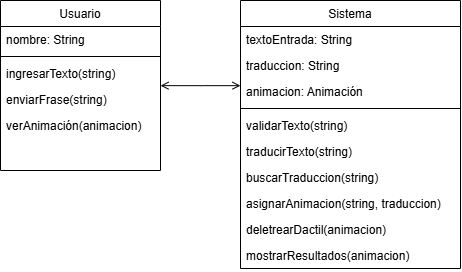
\includegraphics[width=0.6\textwidth]{Images/Cap 3/clases.png}
    \captionof{figure}{Diagrama de clases del sistema.} 
\end{center}

\subsection{Diagrama de secuencia}
\begin{center}
    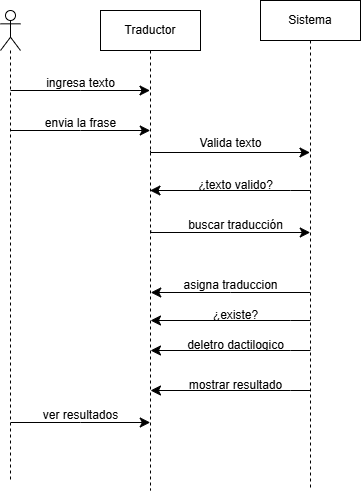
\includegraphics[width=0.6\textwidth]{Images/Cap 3/secuencia.png}
    \captionof{figure}{Diagrama de secuencia del sistema.}
\end{center}
\subsection{Requerimientos no funcionales}
\begin{itemize}
    \item \textbf{RnF01: Rendimiento}  
    La aplicación debe cargar y procesar las traducciones en menos de 2 segundos, garantizando una experiencia de usuario rápida y eficiente.
    
    \item \textbf{RnF02: Usabilidad}  
    La interfaz debe ser fácil de navegar, con instrucciones claras y botones de acción bien definidos, siguiendo las heurísticas de usabilidad de Nielsen.
    
    % \item \textbf{RnF03: Seguridad}  
    % La aplicación debe proteger los datos del usuario mediante cifrado y garantizar que no se almacenen datos sensibles sin el consentimiento explícito del usuario.
    
    \item \textbf{RnF03: Escalabilidad}  
    El sistema debe ser capaz de adaptarse a futuras expansiones, como la inclusión de más frases, soporte para otros dialectos de señas o integración con otras plataformas.
\end{itemize}
\subsection{Casos de uso}
\subsubsection{Caso de uso 01: Entrada de texto}
\subsubsection{Resumen}
El usuario ingresa texto en español en la aplicación, que luego es procesado y traducido a LSM.
\subsubsection{Descripción}
\begin{table}[h]
    \centering
    \begin{longtable}{|l|p{10cm}|}  % La segunda columna usa p{10cm} para ajustar el texto
    \hline
    \textbf{Atributos} & Tipo de texto: Español, límite de 500 caracteres, validación de caracteres permitidos. \\ \hline
    \textbf{Actores} & Usuario (quien ingresa el texto). \\ \hline
    \textbf{Precondiciones} & El sistema está abierto y funcionando correctamente. El usuario debe estar en la pantalla principal. \\ \hline
    \textbf{Actividad que se va a bitácora} & Registro del texto ingresado por el usuario y la fecha y hora de la traducción solicitada. \\ \hline
    \textbf{Registro que se va a bitácora} & Texto ingresado, usuario que lo ingresó, IP del dispositivo, timestamp de la acción. \\ \hline
    \textbf{Viene de} &  \\ \hline    
    \end{longtable}
\end{table}
    

\subsubsection{Trayectoria principal}
\begin{enumerate}[label=\textbf{\arabic*}, leftmargin=1.5cm]
    \item \UCsystem \ El sistema muestra un campo de entrada de texto en la pantalla principal de la aplicación, permitiendo al usuario ingresar texto en español.  
    Además, la interfaz incluye:  
    \begin{itemize}
        \item Botón para iniciar la traducción.
    \end{itemize}

    \item \UCactor \ Ingresa el texto en el campo de entrada.  
   
    \item \UCsystem \ El sistema procesa el texto ingresado y lo traduce a LSM, mostrando el resultado en formato animado o en video.

    \item \UCactor \ Puede modificar el texto y volver a ejecutar la traducción si es necesario.

\end{enumerate}

\textit{--- Fin del caso de uso.}

\subsubsection{Diseño de la interfaz}

\subsubsection{Caso de uso 02: Procesamiento de Lenguaje Natural (PLN)}
\subsubsection{Resumen}
El sistema procesa el texto ingresado mediante PLN y lo prepara para su conversión a señas en LSM.
\subsubsection{Descripción}
\begin{table}[h]
    \centering
    \begin{longtable}{|l|p{10cm}|}  % La segunda columna usa p{10cm} para ajustar el texto
    \hline
    \textbf{Atributos} & Tipo de texto procesado, análisis semántico y sintáctico. \\ \hline
    \textbf{Actores} & Sistema (encargado del procesamiento del texto). \\ \hline
    \textbf{Precondiciones} & El texto ingresado por el usuario debe estar disponible y correctamente formateado. \\ \hline
    \textbf{Actividad que se va a bitácora} & Registro del texto procesado, las frases clave y el análisis semántico realizado. \\ \hline
    \textbf{Registro que se va a bitácora} & Texto procesado, identificaciones de frases clave, timestamp del análisis. \\ \hline
    \textbf{Viene de} & El caso de uso “Entrada de texto”. \\ \hline
      
    \end{longtable}
\end{table}
    
\subsubsection{Trayectoria principal}
\begin{enumerate}[label=\textbf{\arabic*}, leftmargin=1.5cm]
    \item \UCsystem \ El sistema recibe el texto ingresado por el usuario.
    
    \item \UCsystem \ El sistema analiza el texto utilizando el módulo de procesamiento de lenguaje natural, identificando frases clave y contexto semántico para una traducción adecuada.
    
    \item \UCsystem \ El sistema prepara el texto procesado para la generación de las señas en LSM.

\end{enumerate}

\textit{--- Fin del caso de uso.}
\newpage
\subsubsection{Caso de uso 03: Generación de Avatares 3D}
\subsubsection{Resumen}
El sistema genera un avatar 3D que realiza y muestra en pantalla la traducción en señas LSM, incluyendo expresiones faciales y movimientos corporales.
\subsubsection{Descripción}
\begin{table}[h]
    \centering
    \begin{longtable}{|l|p{10cm}|}  % La segunda columna usa p{10cm} para ajustar el texto
    \hline
    \textbf{Atributos} & Avatar 3D, animación de señas, expresiones faciales y movimientos corporales. \\ \hline
    \textbf{Actores} & Sistema (generador del avatar 3D), Usuario (quien visualiza el avatar). \\ \hline
    \textbf{Precondiciones} & El texto debe haber sido procesado y traducido a LSM correctamente. \\ \hline
    \textbf{Actividad que se va a bitácora} & Registro de la generación del avatar y las animaciones realizadas. \\ \hline
    \textbf{Registro que se va a bitácora} & Avatar generado, tipo de señas representadas, timestamp de la generación. \\ \hline
    \textbf{Viene de} & El caso de uso “Procesamiento de Lenguaje Natural (PLN)”. \\ \hline
       
    \end{longtable}
\end{table}
    
\subsubsection{Trayectoria principal}
\begin{enumerate}[label=\textbf{\arabic*}, leftmargin=1.5cm]
    \item \UCsystem \ El sistema genera un avatar 3D correspondiente a la traducción de la frase en LSM.
    
    \item \UCsystem \ El avatar 3D realiza las señas correspondientes, incluyendo expresiones faciales y movimientos corporales.

    \item \UCsystem \ El avatar 3D se presenta en la pantalla al usuario, mostrando la traducción de la frase en LSM.

\end{enumerate}

\textit{--- Fin del caso de uso.}
\newpage
\subsubsection{Caso de uso 04: Modo de Deletreo}
\subsubsection{Resumen}
El sistema detecta una palabra desconocida y activa el modo de deletreo, mostrando cada letra con gestos del alfabeto dactilológico de LSM.
\subsubsection{Descripción}
\begin{table}[h]
    \centering
    \begin{longtable}{|l|p{10cm}|}  % La segunda columna usa p{10cm} para ajustar el texto
    \hline
    \textbf{Atributos} & Alfabeto dactilológico, letras individualmente representadas en LSM. \\ \hline
    \textbf{Actores} & Usuario (quien observa el deletreo), Sistema (que activa el modo de deletreo). \\ \hline
    \textbf{Precondiciones} & La palabra no debe estar en la base de datos de LSM. \\ \hline
    \textbf{Actividad que se va a bitácora} & Registro del uso del modo de deletreo por parte del usuario. \\ \hline
    \textbf{Registro que se va a bitácora} & Palabra deletreada, secuencia de letras, timestamp de la actividad. \\ \hline
    \textbf{Viene de} & El caso de uso “Entrada de texto” o “Procesamiento de Lenguaje Natural (PLN)”. \\ \hline
     
    \end{longtable}
\end{table}
  
\subsubsection{Trayectoria principal}
\begin{enumerate}[label=\textbf{\arabic*}, leftmargin=1.5cm]
    \item \UCsystem \ El sistema detecta que la palabra ingresada no está en la base de datos de LSM.
    
    \item \UCsystem \ El sistema activa el modo de deletreo, permitiendo al usuario ver la palabra deletreada utilizando el alfabeto dactilológico de LSM.
    
    \item \UCactor \ El usuario observa las letras del deletreo en la pantalla, cada una representada por un gesto del alfabeto dactilológico de LSM.

\end{enumerate}

\textit{--- Fin del caso de uso.}
\newpage
\subsubsection{Caso de uso 05: Animaciones y Transiciones}
\subsubsection{Resumen}
El sistema usa IA para gestionar animaciones fluidas entre señas en LSM, evitando movimientos bruscos y mejorando la experiencia visual.
\subsubsection{Descripción}
\begin{table}[h]
    \centering
    \begin{longtable}{|l|p{10cm}|}  % La segunda columna usa p{10cm} para ajustar el texto
    \hline
    \textbf{Atributos} & Animación fluida, transiciones entre señas optimizadas, uso de IA. \\ \hline
    \textbf{Actores} & Sistema (que gestiona las animaciones y transiciones). \\ \hline
    \textbf{Precondiciones} & El avatar 3D debe estar generado y las señas deben estar listas para la animación. \\ \hline
    \textbf{Actividad que se va a bitácora} & Registro de la generación y ejecución de las animaciones y transiciones. \\ \hline
    \textbf{Registro que se va a bitácora} & Transiciones entre señas, optimización de IA, timestamp de la animación. \\ \hline
    \textbf{Viene de} & El caso de uso “Generación de Avatares 3D”. \\ \hline
      
    \end{longtable}
\end{table}
    
\subsubsection{Trayectoria principal}
\begin{enumerate}[label=\textbf{\arabic*}, leftmargin=1.5cm]
    \item \UCsystem \ El sistema gestiona las animaciones entre las señas de LSM, asegurando que sean fluidas y naturales.
    
    \item \UCsystem \ Utiliza inteligencia artificial (IA) para optimizar las transiciones entre las señas, evitando movimientos bruscos o poco realistas.
    
    \item \UCsystem \ El sistema presenta las animaciones de las señas con transiciones suaves, brindando una experiencia visual coherente.

\end{enumerate}

\textit{--- Fin del caso de uso.}
\newpage
\subsubsection{Caso de uso 06: Compatibilidad}
\subsubsection{Resumen}
La aplicación es compatible con la última versión de Android y se adapta a diversos dispositivos y tamaños de pantalla.
\subsubsection{Descripción}
\begin{table}[h]
    \centering
    \begin{longtable}{|l|p{10cm}|}  % La segunda columna usa p{10cm} para ajustar el texto
    \hline
    \textbf{Atributos} & Compatibilidad con versiones de Android, ajustes automáticos según dispositivos. \\ \hline
    \textbf{Actores} & Sistema (que garantiza la compatibilidad), Usuario (que utiliza la aplicación). \\ \hline
    \textbf{Precondiciones} & La aplicación debe estar instalada en un dispositivo con la versión compatible de Android. \\ \hline
    \textbf{Actividad que se va a bitácora} & Registro de la versión de Android y la compatibilidad del dispositivo. \\ \hline
    \textbf{Registro que se va a bitácora} & Versión de Android, tipo de dispositivo, timestamp de la verificación de compatibilidad. \\ \hline
    \textbf{Viene de} & El caso de uso “Inicio de la aplicación” o “Verificación de configuración del dispositivo”. \\ \hline
       
    \end{longtable}
\end{table}
    
\subsubsection{Trayectoria principal}
\begin{enumerate}[label=\textbf{\arabic*}, leftmargin=1.5cm]
    \item \UCsystem \ La aplicación debe ser compatible con la última versión de Android.
    
    \item \UCsystem \ El sistema garantiza su funcionamiento en una amplia gama de dispositivos móviles, ajustándose a diferentes tamaños de pantalla y capacidades del dispositivo.

\end{enumerate}

\textit{--- Fin del caso de uso.}
\newpage
\begin{longtable}{|p{5cm}|p{5cm}|p{5cm}|}
    \hline
    \textbf{Emergencia (3 a 5 palabras)} & \textbf{Saludo (2 a 4 palabras)} & \textbf{Agradecimiento
    /Respuestas (2 a 4 palabras)} \\ \hline
    \endfirsthead
    \hline
    \textbf{Emergencia (3 a 5 palabras)} & \textbf{Saludo (2 a 4 palabras)} & \textbf{Agradecimiento/Respuestas (2 a 4 palabras)} \\ \hline
    \endhead
    \hline
    Ayuda, por favor. & Hola, ¿cómo estás? & Gracias. \\
    Llama a la policía. & Buenos días. & Muchas gracias. \\
    Necesito un médico. & Buenas tardes. & Te lo agradezco. \\
    Estoy herido/a. & Buenas noches. & Que amable. \\
    ¿Dónde está el hospital? & ¿Qué tal? & Estoy muy agradecido/a. \\
    Es una emergencia. & Mucho gusto. & Gracias por tu ayuda. \\
    ¿Puedes ayudarme? & Encantado/a de conocerte. & Cuando quieras. \\
    Necesito asistencia urgente. & ¿Cómo te llamas? & No hay problema. \\
    ¿Dónde está la salida? & Me llamo [nombre]. & No pasa nada. \\
    ¡Fuego! ¡Fuego! & Hasta luego. & Es un placer. \\
    \hline
    \end{longtable}


\subsection{Diagrama de casos de uso}
\subsection{Mockups del sistema}
\subsection{Identificación de riesgos}
\subsection{Evaluación de riesgos}
\subsection{Mitigación de riesgos}

\section{Selección de los datos}
\subsection{Recolección de datos}

\section{Preparación de los datos}

\chapter{Conclusiones}

\chapter{Referencias}


\chapter{Trabajo relacionado}

\chapter{Desarrollo}

\chapter{Experimentos}

\chapter{Conclusiones y trabajo futuro}